\chapter{eTrice Models and Their Relations}

eTrice comprises several models:

\begin{itemize}
\item the ROOM model (*.room) -- defines model classes and the logical structure of the model
\item Config model (*.config) -- defines configuration values for attributes
\item Physical model (*.etphys) -- defines the structure and properties of the physical system
\item Mapping model (*.etmap) -- defines a mapping from logical elements to physical elements
\end{itemize}

In the following diagram the models and their relations are depicted. The meaning of the arrows is: uses/references.

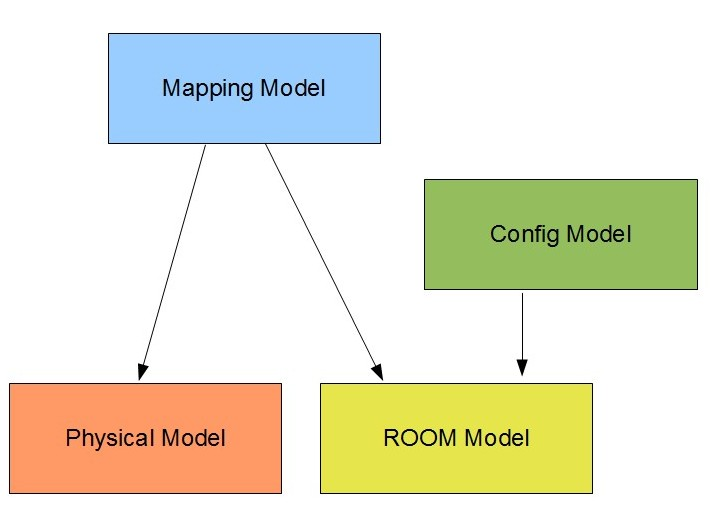
\includegraphics[scale=0.4]{images/080-models.jpg}
% !{width:50}images/080-models.jpg!

In the following sections we will describe those models with emphasis of their cross relations.

\section{The ROOM Model}

The ROOM model defines classes for Data, Protocols, Actors, SubSystems and LogicalSystems.
Thereby the three latter form a hierarchy. The @LogicalSystem@ is the top level element of the structure. It contains references to \texttt{SubSystemClass} elements. The \texttt{SubSystemClass} in turn contain references to \texttt{ActorClass} elements which again contain (recursively) references to \texttt{ActorClass} elements. The complete structural hierarchy implies a tree which has the \texttt{LogicalSystem} as root and where each reference stands for a new node with possibly further branches.

Let's consider a simple example. It doesn't implement any meaningful and completely omits behavioral and other aspects.

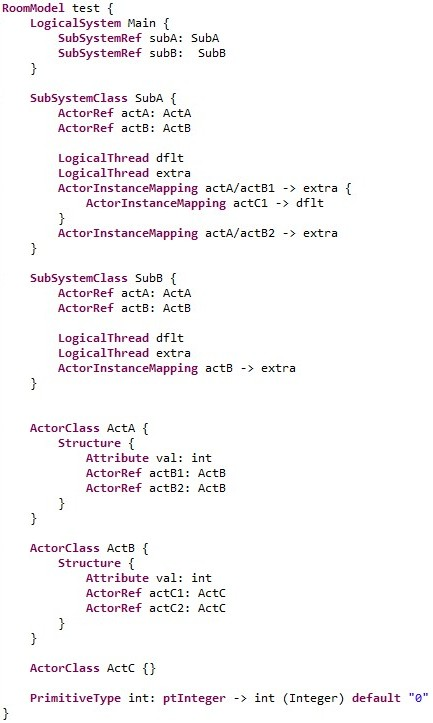
\includegraphics{images/080-room.jpg}
% !images/080-room.jpg!

When a \texttt{LogicalSstem} is instantiated then recursively all of the contained referenced elements are instantiated as instances of the corresponding class. Thus the instance tree of above example looks like this (the third line in the white boxes shows some mapping information, s.b.):

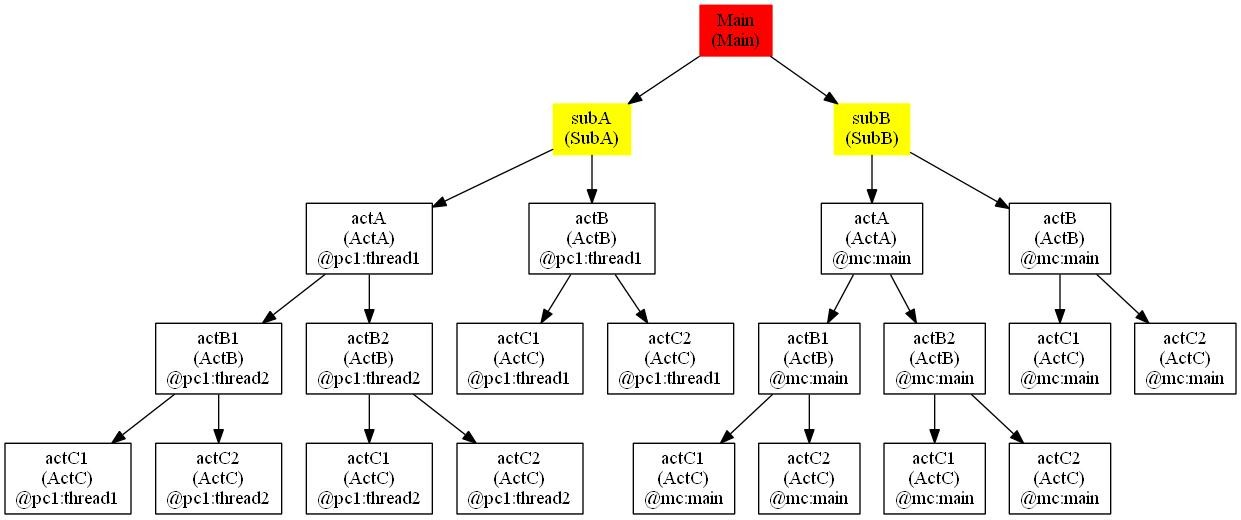
\includegraphics[scale=0.35]{images/080-instances.jpg}
% !{width:40%}images/080-instances.jpg!


\section{The Config Model}

Once we have the ROOM class model we can configure values using the Config model. This can be done on the class level and/or on the instance level. Values defined for class attributes are used for all instances unless there is an instance value configured for the same attribute.

!images/080-config.jpg!

\section{The Physical Model}

The physical model defines the physical resources onto which the logical system will be deployed. It is possible to define runtime classes which (currently) only defines the overall execution model of the platform.

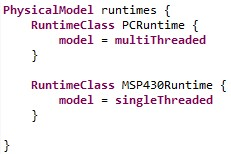
\includegraphics{images/080-runtimes.jpg}
% !images/080-runtimes.jpg!

The physical system is composed of @Node@ references where each @Node@ is defined as a class referencing a @RuntimeClass@ and defining @Threads@.

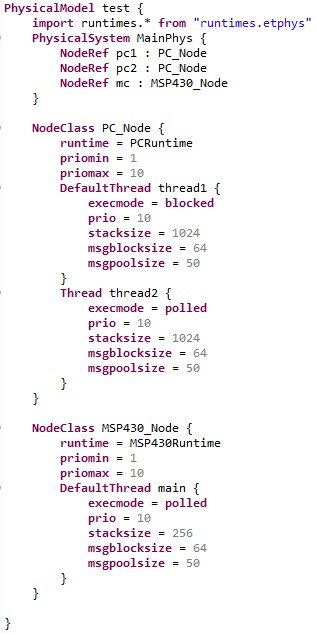
\includegraphics{images/080-phys.jpg}
% !images/080-phys.jpg!

\section{The Mapping Model}

The last model finally combines all this information by mapping logical to physical entities.

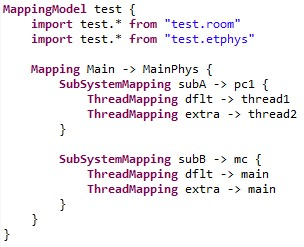
\includegraphics{images/080-map.jpg}
% !images/080-map.jpg!

The result of the mapping is also depicted in above tree diagram of the instances. All actor instances (the white boxes) are mapped to a node and a thread running on this node (shown as @ \textit{node} : \textit{thread}).
